\documentclass[conference]{IEEEtran}
\IEEEoverridecommandlockouts

\usepackage{cite}
\usepackage{amsmath,amssymb,amsfonts}
\usepackage{graphicx}
\usepackage{xcolor}
\usepackage{tikz}
\usetikzlibrary{arrows.meta,positioning,fit,backgrounds,calc}
\usepackage[hidelinks]{hyperref}
\usepackage{url}

\begin{document}

\title{Valence-Selective Transfer in Frozen Speech-Emotion Embeddings\\
for Multilingual Voice-Based Stress Detection}

\author{}

\maketitle

\begin{abstract}
Voice-based stress detectors increasingly reuse frozen speech-emotion (SER)
embeddings, and the checkpoint is usually chosen by how well it agrees with acted
emotional speech in-domain. We find that this criterion \emph{reverses} on real,
spontaneous stress: over six fusion checkpoints, stronger in-domain arousal
agreement goes with \emph{weaker} real-voice accuracy (Spearman $\rho = -0.60$),
and the checkpoint the convention would reject ($0.35$ in-domain) is the one that
deploys best ($91.7\%$ leave-one-out). The reason is a split in what the frozen
embeddings preserve: they retain the \emph{valence} of real stress but lose its
\emph{arousal}. On held-out real clips, stressed speech reads as correctly
negative in valence $82$--$100\%$ of the time yet correctly high in arousal only
$12$--$53\%$ of the time. The same gap reappears on a large independent corpus
(IEMOCAP, $n = 2{,}132$), where predicted valence tracks the labels far more
closely than arousal ($r = 0.688$ vs.\ $0.485$; bootstrap intervals on the
per-clip difference clear zero for every out-of-domain checkpoint). A
matched-size probe shows this is an effect of emotion pretraining rather than
capacity: at equal width emotion2vec encodes valence much better than WavLM
(CCC $0.660$ vs.\ $0.387$), while WavLM leans toward arousal instead---so the
valence advantage is encoder-specific. Following the diagnosis, a
\emph{valence-primary} scoring rule widens the stressed/calm gap over the usual
arousal-based rule for every checkpoint (Cohen's $d = 1.71$). We ship the result
as a bilingual detector for English and Sinhala that hands arousal magnitude to a
physiological module by design, and we state plainly where a frozen encoder
fails out of distribution.
\end{abstract}

\begin{IEEEkeywords}
voice stress detection, speech emotion recognition, valence and arousal,
frozen embeddings, emotion2vec, prosody, multilingual, low-resource,
affective computing.
\end{IEEEkeywords}

\section{Introduction}

Speech carries reliable traces of psychological stress, and reading stress from
the voice is appealing because it is passive, cheap, and needs nothing more than
a microphone. In well-being systems that adapt \emph{as a session unfolds}---say a
meditation environment that responds to how stressed a student or desk-worker is
right now---the voice is often the only affective signal on hand without extra
wearables. The real question is therefore not whether stress leaves a vocal trace,
but whether it can be read \emph{reliably from a few seconds of real, spontaneous
speech} by an unseen speaker, in more than one language, and without gathering a
large labelled in-domain corpus first.

The standard fix for the data problem is a \emph{frozen} SER encoder.
Self-supervised and emotion-pretrained models---wav2vec\,2.0~\cite{wav2vec2},
WavLM~\cite{wavlm}, emotion2vec~\cite{emotion2vec}---provide a fixed
high-dimensional representation that a small head maps to affect, so only a few
hundred thousand parameters need training instead of a 300M-parameter backbone.
Since affect is conventionally placed in the two-dimensional
\emph{valence--arousal} plane of the circumplex model~\cite{russell1980}, these
heads are trained as regressors on valence and arousal and scored with the
concordance correlation coefficient (CCC)~\cite{lin1989ccc}. The resulting habit
is rarely stated but widely followed: \emph{pick the checkpoint with the highest
in-domain valence/arousal CCC and expect it to deploy best.} It is a convenient
habit, because in-domain CCC is cheap to measure on the acted benchmarks these
models are trained on---IEMOCAP~\cite{iemocap}, MELD~\cite{meld}, and the like.

The habit assumes something that has not been checked: that matching \emph{acted}
emotional speech predicts accuracy on \emph{real} stress. Acted corpora are voiced
by performers told to portray an emotion, and they lean heavily toward the loud,
high-arousal corner of the space~\cite{douglascowie2003}. Real stress---in
students and desk-workers especially---often shows up instead as a quiet,
flattened ``freeze'': negative in valence but \emph{low} in arousal. If what a
frozen encoder carries over from acted data is not what separates real stress,
then ranking checkpoints by in-domain CCC may be useless---or worse, backwards. As
far as we know this has not been tested directly for real-voice deployment: a
distribution shift can drag down overall accuracy without revealing \emph{which}
affective axis actually survives it.

We test it directly. With six fusion checkpoints spanning the acted-to-natural
range, a held-out set of real stressed and calm clips, and a large independent
corpus for replication, we ask whether in-domain accuracy predicts real-voice
accuracy---and if not, why. The result is a clean negative with a mechanism behind
it. First, the criterion does not just fail to predict deployment---it
\emph{inverts} it: across the six checkpoints, higher in-domain arousal CCC comes
with \emph{lower} real-voice accuracy (Spearman $\rho = -0.60$), so the checkpoint
ranked worst by convention ($0.35$ in-domain) deploys best ($91.7\%$ leave-one-out).
Second, the inversion has a definite cause: frozen embeddings preserve the
\emph{valence} of real stress but not its \emph{arousal}. On real stressed clips
valence is correctly negative $82$--$100\%$ of the time while arousal is correctly
high only $12$--$53\%$ of the time; the same asymmetry replicates on IEMOCAP
($n = 2{,}132$), where predicted valence tracks the labels much better than
arousal ($r = 0.688$ vs.\ $0.485$) and the bootstrap interval on the difference
clears zero for every out-of-domain checkpoint. Fig.~\ref{fig:concept} sketches
the picture: the valence axis that tells real stress from calm survives, while the
arousal axis on which real ``freeze'' stress differs from acted stress collapses.

The diagnosis leads straight to an action. If valence is what the embeddings
recover for real stress, then stress should be read \emph{from valence}, not from
arousal. A valence-primary rule widens the stressed/calm gap over the arousal-based
rule on all six checkpoints, with a large effect (Cohen's $d = 1.71$). With a
matched-size probe we further show the valence edge comes from \emph{emotion
pretraining}, not model size: at equal width emotion2vec carries valence far
better than WavLM (CCC $0.660$ vs.\ $0.387$), whereas WavLM tilts the other way,
toward arousal. The split is thus encoder-specific---which is exactly why
valence-primary scoring on an emotion-pretrained encoder is a design choice, not a
universal rule.

Because our target is bilingual, we test in English and Sinhala. English, well
covered by the encoder's pretraining, separates strongly; Sinhala, a low-resource
language absent from it~\cite{sinhala_openslr}, marks the honest limit of a frozen
encoder out of distribution---one that more in-language data does not lift. The
deployed system handles this by design: arousal magnitude, which the voice does
not supply dependably, is handed to a separate physiological
(heart-rate-variability) module, and the voice contributes only the valence-driven
estimate it can support. The paper is therefore diagnosis and design together: why
a common selection habit fails on real stress, and what to do instead.

\medskip
\noindent\textbf{Contributions.}
\begin{itemize}
  \item We show that ranking frozen SER models by in-domain acted CCC is
  \emph{anti-correlated} with real-voice stress accuracy (Spearman
  $\rho = -0.60$), reversing a common selection habit.
  \item We trace the cause to a \emph{valence--arousal split}---frozen emotion
  embeddings carry the valence of real stress but not its arousal---and replicate
  it at scale on IEMOCAP ($n = 2{,}132$) with bootstrap significance.
  \item We show the split is \emph{encoder-specific} to emotion pretraining with a
  matched-size probe (emotion2vec vs.\ WavLM), not an artefact of size or
  architecture.
  \item We derive and validate a \emph{valence-primary} scoring rule that follows
  from the diagnosis and widens stressed/calm separation on every checkpoint
  (Cohen's $d = 1.71$), deployed as a bilingual (English/Sinhala) detector that
  defers arousal to a physiological module.
  \item We report the negative and limiting results plainly---the small-sample and
  out-of-distribution Sinhala limits, including a controlled case where adding
  in-language data \emph{hurt} accuracy---as findings in their own right.
\end{itemize}

\begin{figure}[t]
\centering
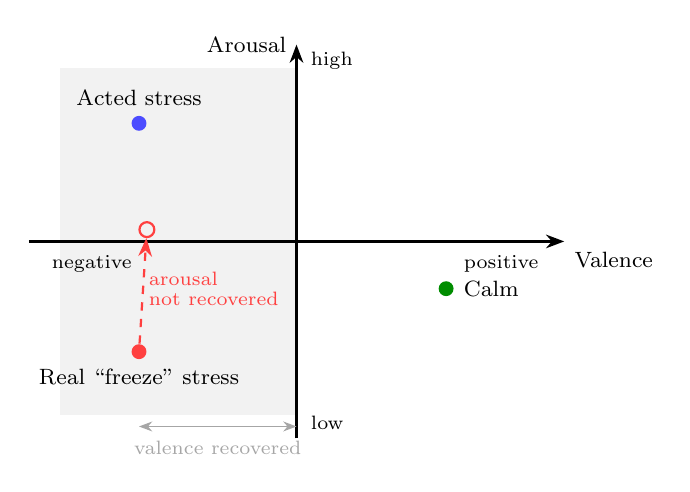
\begin{tikzpicture}[>=Stealth, font=\footnotesize]
  \fill[gray!10] (-3,-2.2) rectangle (0,2.2);
  \draw[->,thick] (-3.4,0) -- (3.4,0) node[below right] {Valence};
  \draw[->,thick] (0,-2.5) -- (0,2.5) node[left] {Arousal};
  \node[below] at (2.6,-0.05) {\scriptsize positive};
  \node[below] at (-2.6,-0.05) {\scriptsize negative};
  \node[right] at (0.06,2.3) {\scriptsize high};
  \node[right] at (0.06,-2.3) {\scriptsize low};
  \node[circle,fill=blue!70,inner sep=1.9pt,label={above:{Acted stress}}] (as) at (-2,1.5) {};
  \node[circle,fill=red!75,inner sep=1.9pt,label={below:{Real ``freeze'' stress}}] (rs) at (-2,-1.4) {};
  \node[circle,fill=green!55!black,inner sep=1.9pt,label={right:{Calm}}] (ca) at (1.9,-0.6) {};
  \node[circle,draw=red!75,thick,inner sep=1.9pt] (rsp) at (-1.9,0.15) {};
  \draw[->,red!75,dashed,thick] (rs) -- (rsp);
  \node[red!75,align=left] at (-1.05,-0.6) {\scriptsize arousal\\[-2pt]\scriptsize not recovered};
  \draw[<->,gray!70] (-2,-2.35) -- (0,-2.35);
  \node[gray!70] at (-1,-2.62) {\scriptsize valence recovered};
\end{tikzpicture}
\caption{The valence--arousal split (schematic). Both acted and real ``freeze''
stress are negative in valence, but acted stress sits high in arousal while real
freeze stress sits low. Frozen embeddings keep the \emph{valence} (horizontal)
gap between real stress and calm, yet pull its \emph{arousal} (vertical) gap toward
neutral (dashed arrow): valence survives, arousal does not. This is what motivates
the valence-primary rule in the deployed detector.}
\label{fig:concept}
\end{figure}

\section{Related Work}

\textbf{Frozen speech representations.} Self-supervised encoders learn
general-purpose features from unlabelled audio and are now the default front-end
for speech tasks. wav2vec\,2.0~\cite{wav2vec2} and WavLM~\cite{wavlm} optimise
masked-prediction or contrastive objectives on large collections and are commonly
used with a frozen backbone under a lightweight probe. emotion2vec~\cite{emotion2vec}
adapts this recipe to affect, pretraining on emotional speech so its features
track emotion rather than phonetic content, and recent transfer systems reuse such
embeddings---at times alongside speaker vectors---as fixed features for
classification~\cite{jakubec2024}. We use a frozen emotion2vec encoder in this same
probe-on-top setting, but ask a question the benchmarks do not: when deployment
departs sharply from acted training data, \emph{which} affective axis a frozen
encoder still supports.

\textbf{Dimensional emotion and its evaluation.} The valence--arousal
circumplex~\cite{russell1980} underlies most affect models, and continuous
recognition is typically scored with CCC~\cite{lin1989ccc} against valence and
arousal on acted corpora such as IEMOCAP~\cite{iemocap} and MELD~\cite{meld}. That
acted and naturalistic emotion differ in both distribution and
recoverability~\cite{douglascowie2003} is well established and motivates our
question; but this line of work tends to treat the two axes symmetrically when
transfer is poor, whereas we show the failure is asymmetric and axis-specific.

\textbf{Voice-based stress in the wild.} Reading affect and stress from real speech
has a long history, often with prosody-centred feature sets such as
GeMAPS~\cite{gemaps}. Nearest to us, EMOVOME~\cite{emovome} recognises emotion from
spontaneous voice messages by fusing pretrained embeddings with eGeMAPS features,
and reports that spontaneous speech trails acted corpora while matching elicited
data. That work, like ours, establishes that real speech is not acted speech; our
addition is to explain the failure---valence transfers, arousal does not---and to
turn it into a concrete selection-and-scoring rule rather than an accuracy figure.
More broadly, such systems read stress as a high-arousal state, an assumption our
results complicate for internalised stress, where the arousal cue is faint and
valence is the dependable signal.

\textbf{Multilingual and low-resource SER.} Multilingual SER has been approached
with transformers trained under augmentation and cross-corpus fusion
\cite{multiling_ser}, and cross-lingual pretraining helps languages seen in
training. Genuinely under-resourced languages---Sinhala among
them~\cite{sinhala_openslr}---still fall out of distribution for encoders trained
mostly on high-resource speech. Against the augmentation-helps narrative, we report
a controlled case where adding in-language Sinhala data \emph{lowered} held-out
accuracy, and so treat Sinhala not as a solved multilingual case but as a
controlled probe of frozen-encoder behaviour out of distribution.

\textbf{Position.} Our contribution is diagnostic. We propose no new encoder or
benchmark; we show a common selection convention is not merely uninformative but
inverted on real stress, explain the inversion through a valence--arousal split we
replicate at scale, and derive the scoring rule that follows from it.

\section{Method}

\subsection{Data}
The real-voice set is $n = 24$ held-out clips ($17$ stressed, $7$ calm) from
consenting speakers---$13$ English and $11$ Sinhala from roughly three speakers.
Every split here is speaker-independent. For large-$n$ replication we use $2{,}132$
held-out IEMOCAP~\cite{iemocap} utterances, each with continuous valence and
arousal labels. The six fusion checkpoints differ only in training corpus and so
span the acted-to-natural range: Fusion-Acted (acted emotion), Fusion-V2,
Fusion-Combined, Fusion-Augmented, Fusion-IEMOCAP (in-domain on IEMOCAP), and
Fusion-MELD (the shipped model, trained on the naturalistic conversational MELD
corpus~\cite{meld}).

\subsection{Model}
Fig.~\ref{fig:arch} gives the architecture. Audio passes through a frozen
emotion2vec-plus-large encoder~\cite{emotion2vec} ($\sim$300M parameters, feature
extractor only) yielding a $1024$-d embedding $\mathbf{e}_0$, and through a
prosodic front-end computing $21$ interpretable features $\mathbf{p}_0$ (pitch
statistics, jitter, shimmer, harmonics-to-noise ratio, RMS energy, zero-crossing
rate, spectral centroid/rolloff/flatness, speech rate, pause ratio, voiced
fraction, duration) in the spirit of GeMAPS~\cite{gemaps}. A gated fusion
head---the only trainable part ($\sim$1--2M parameters)---mixes the two streams and
regresses valence and arousal:
\begin{equation}
\begin{gathered}
\mathbf{e} = \mathrm{ReLU}(\mathrm{LN}(\mathbf{W}_e\mathbf{e}_0)),\quad
\mathbf{p} = \mathrm{ReLU}(\mathrm{LN}(\mathbf{W}_p\mathbf{p}_0)),\\[2pt]
\mathbf{g} = \sigma(\mathbf{W}_g[\mathbf{e};\mathbf{p}]),\quad
\mathbf{f} = \mathbf{g}\odot\mathbf{e} + (1-\mathbf{g})\odot\mathbf{p},\\[2pt]
(\hat{v},\hat{a}) = \tanh(\mathrm{head}(\mathbf{f})).
\end{gathered}
\end{equation}
Here $\mathbf{W}_e\!:\!1024\!\to\!128$ and $\mathbf{W}_p\!:\!21\!\to\!128$, the
gate $\mathbf{g}\in(0,1)^{128}$ mixes streams elementwise, and the head maps
$128\!\to\!64\!\to\!\mathrm{ReLU}\!\to\!\mathrm{Dropout}(0.3)\!\to\!2$ to
$\hat{v},\hat{a}\in(-1,1)$. Only the head, fusion, and prosody projections
train---the encoder stays frozen---under a concordance loss with a small MSE term,
$\mathcal{L} = 1 - \tfrac{1}{2}(\mathrm{CCC}_v + \mathrm{CCC}_a) +
0.2\,\mathrm{MSE}$.

\begin{figure}[t]
\centering
\resizebox{\columnwidth}{!}{%
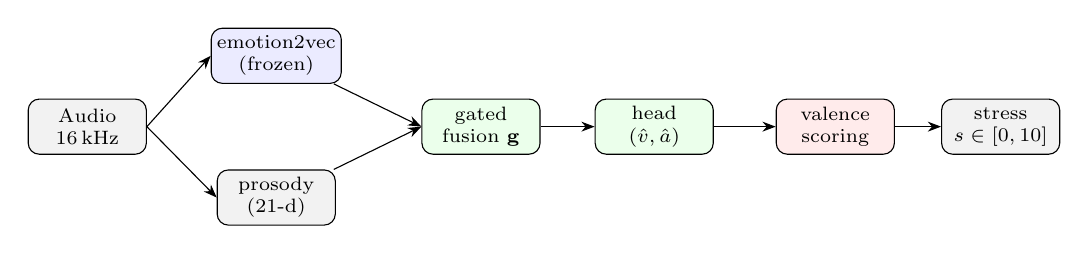
\begin{tikzpicture}[
   >=Stealth, font=\scriptsize,
   box/.style={draw, rounded corners, minimum height=7mm, minimum width=15mm,
               align=center, inner sep=2pt},
   frozen/.style={box, fill=blue!8},
   train/.style={box, fill=green!8},
   io/.style={box, fill=gray!10}]
  \node[io]     (audio) at (0,0)      {Audio\\16\,kHz};
  \node[frozen] (enc)   at (2.4,0.9)  {emotion2vec\\(frozen)};
  \node[io]     (pros)  at (2.4,-0.9) {prosody\\(21-d)};
  \node[train]  (gate)  at (5.0,0)    {gated\\fusion $\mathbf{g}$};
  \node[train]  (head)  at (7.2,0)    {head\\$(\hat v,\hat a)$};
  \node[box, fill=red!8] (score) at (9.5,0) {valence\\scoring};
  \node[io]     (out)   at (11.6,0)   {stress\\$s\in[0,10]$};
  \draw[->] (audio.east) -- (enc.west);
  \draw[->] (audio.east) -- (pros.west);
  \draw[->] (enc)  -- (gate.west);
  \draw[->] (pros) -- (gate.west);
  \draw[->] (gate)  -- (head);
  \draw[->] (head)  -- (score);
  \draw[->] (score) -- (out);
\end{tikzpicture}}
\caption{System architecture. The 300M-parameter emotion2vec encoder is frozen and
used only as a feature extractor; the prosodic front-end and gated fusion head
(blue = frozen, green = trained, $\sim$1--2M parameters) are the only trained
parts. The head predicts valence and arousal, but only valence drives the deployed
score.}
\label{fig:arch}
\end{figure}

\subsection{Scoring}
The legacy rule reads stress off arousal; our \emph{valence-primary} rule reads it
off valence, $s = \mathrm{round}(10\max(0,-\hat{v}),\,2)\in[0,10]$ with confidence
$c = \min(1,|\hat{v}|)$. A clip is flagged stressed when $s > 2.0$, a threshold set
by leave-one-out validation. Arousal magnitude is deliberately not used as a stress
magnitude; the system hands it to a separate heart-rate-variability module.

\subsection{Preprocessing}
Training and inference share one pipeline: resample to $16$~kHz mono, a $70$~Hz
high-pass filter, silence trimming, and loudness normalisation to RMS $0.05$. A
lightweight quality gate drops clips that are too quiet, clipped, or short on
detected voice before scoring.

\subsection{Statistical protocol}
Given the small real-voice set, we keep effect estimation and inference apart. On
the $24$ clips and six checkpoints we report effect sizes (Cohen's
$d$~\cite{cohen1988}), Spearman correlations, and bootstrap $95\%$ intervals
($10{,}000$ resamples)~\cite{efron1993}, and we deliberately do \emph{not} treat
the underpowered $p$-values as significant. Inference is carried instead by the
IEMOCAP replication ($n = 2{,}132$). Deployment accuracy uses leave-one-out (LOO)
thresholding, which removes the bias of tuning a threshold on the same clips it is
scored on.

\section{Results}

\subsection{The inversion}
Table~\ref{tab:inversion} and Fig.~\ref{fig:inversion} plot in-domain acted arousal
CCC (the selection criterion) against real-voice accuracy under legacy scoring. The
trend is monotone and \emph{negative}: as in-domain agreement rises, real-voice
accuracy falls (Spearman $\rho = -0.60$). The weakest in-domain checkpoint,
Fusion-MELD ($0.35$), is the strongest deployed ($0.917$); the strongest in-domain,
Fusion-Acted ($0.81$), is the weakest deployed ($0.375$). With five distinct
in-domain points the correlation is directional, not significant---we claim no
significance here---but the ordering is unambiguous and the mechanism below
explains it. Under the shipped valence-primary scoring the inversion eases to
$\rho = -0.50$, since the fix raises every checkpoint's accuracy: the convention is
harmful under legacy scoring and merely uninformative once scoring is corrected.

\begin{table}[t]
\caption{The inversion: in-domain acted arousal CCC versus real-voice accuracy
(legacy scoring, $n=24$). Higher in-domain score $\to$ lower deployed accuracy.}
\label{tab:inversion}
\centering
\setlength{\tabcolsep}{5pt}
\renewcommand{\arraystretch}{1.2}
\resizebox{\columnwidth}{!}{%
\begin{tabular}{|l|c|c|}
\hline
\textbf{Checkpoint} & \textbf{In-domain acted CCC} & \textbf{Real-voice acc.} \\
\hline
Fusion-Acted           & 0.81 & 0.375 \\
\hline
Fusion-V2              & 0.79 & 0.750 \\
\hline
Fusion-Combined        & 0.77 & 0.625 \\
\hline
Fusion-IEMOCAP         & 0.65 & 0.583 \\
\hline
Fusion-MELD (shipped)  & \textbf{0.35} & \textbf{0.917} \\
\hline
\multicolumn{3}{|c|}{Spearman $\rho = -0.60$ (directional; $n=5$)} \\
\hline
\end{tabular}}
\end{table}

\begin{figure}[t]
\centering
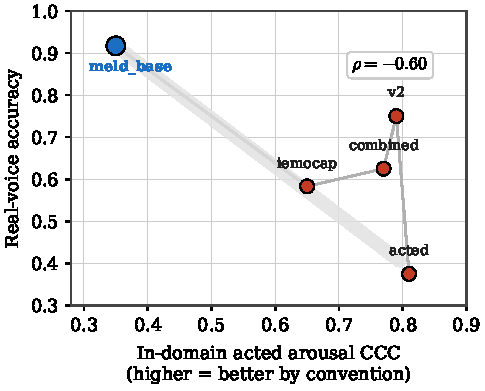
\includegraphics[width=0.82\columnwidth]{figures/fig_inversion.pdf}
\caption{The inversion, visualised. Each point is a checkpoint; the trend falls as
in-domain acted CCC rises. The checkpoint convention would discard (top-left, low
in-domain) deploys best.}
\label{fig:inversion}
\end{figure}

\subsection{The split on real clips}
Separating the two axes exposes the cause. Fig.~\ref{fig:dissociation} shows, on
real stressed clips, how often each checkpoint puts valence on the correct
(negative) side versus arousal on the correct (high) side. Valence is recovered
almost perfectly---$82$ to $100\%$, hitting $100\%$ for the shipped
Fusion-MELD---while arousal is recovered only $12$ to $53\%$ of the time. Real
stress reliably reads as negative in valence but fails to read as high in arousal,
exactly the pattern of Fig.~\ref{fig:concept}: the quiet ``freeze'' of genuine
stress lands in the low-arousal region that acted training never stresses.

\begin{figure}[t]
\centering
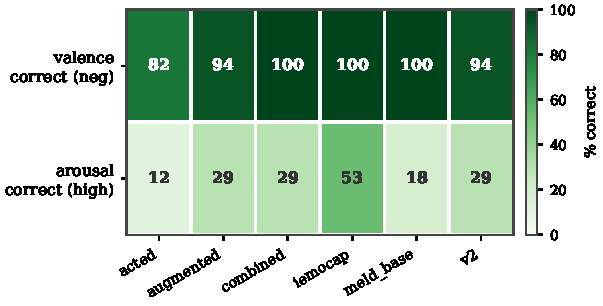
\includegraphics[width=0.92\columnwidth]{figures/fig_dissociation.pdf}
\caption{Valence transfers, arousal does not. On real stressed clips, valence is
correctly negative $82$--$100\%$ of the time; arousal is correctly high only
$12$--$53\%$ of the time, across all six checkpoints.}
\label{fig:dissociation}
\end{figure}

\subsection{Replication on IEMOCAP}
Twenty-four clips cannot support a significance claim, so we replicate the split on
the $2{,}132$-utterance IEMOCAP test set, whose valence and arousal labels let us
correlate predictions with ground truth directly. Table~\ref{tab:iemocap} gives
predicted-versus-true Pearson $r$. For every checkpoint trained \emph{outside}
IEMOCAP, valence correlates well above arousal, and the bootstrap interval on the
per-utterance difference $r_v - r_a$ clears zero in every case---the split is
significant at scale. Two honest nuances follow. First, arousal is \emph{degraded,
not collapsed}, on IEMOCAP: its expressive acted delivery still leaves an arousal
signal ($r_a$ up to $0.62$), whereas the full collapse shows up on quiet real
``freeze'' stress---so the severity of the split scales with how internalised the
stress is. Second, Fusion-IEMOCAP appears only as an upper-bound reference and is
excluded from the replication claim, since it was trained on the distribution it is
evaluated on.

\begin{table}[t]
\caption{IEMOCAP replication ($n=2{,}132$): predicted-versus-true Pearson $r$. For
every out-of-domain checkpoint, valence $\gg$ arousal, and the bootstrap $95\%$
CI on $r_v - r_a$ excludes zero.}
\label{tab:iemocap}
\centering
\setlength{\tabcolsep}{4pt}
\renewcommand{\arraystretch}{1.2}
\begin{tabular}{|l|c|c|c|}
\hline
\textbf{Checkpoint} & $\mathbf{r_v}$ & $\mathbf{r_a}$ & $\mathbf{r_v-r_a}$ \textbf{(95\% CI)} \\
\hline
Fusion-MELD (shipped) & 0.688 & 0.485 & $+0.202$ $[0.159,0.244]$ \\
\hline
Fusion-Acted          & 0.662 & 0.326 & $+0.336$ $[0.293,0.381]$ \\
\hline
Fusion-V2             & 0.674 & 0.404 & $+0.270$ $[0.225,0.314]$ \\
\hline
Fusion-Combined       & 0.726 & 0.621 & $+0.104$ $[0.072,0.140]$ \\
\hline
Fusion-IEMOCAP$^{\dagger}$ & 0.742 & 0.659 & in-domain reference \\
\hline
\end{tabular}
\\[3pt]
{\footnotesize $^{\dagger}$In-domain upper bound; excluded from the replication claim.}
\end{table}

\subsection{The split is encoder-specific}
Is the valence edge from \emph{emotion} pretraining, or just from scale? We answer
with a matched-size ridge probe on IEMOCAP embeddings, comparing emotion2vec and
WavLM at equal width (Table~\ref{tab:encoder}, Fig.~\ref{fig:encoder}). At $1024$
dimensions emotion2vec carries valence far better than WavLM-large (CCC $0.660$
vs.\ $0.387$), and the same holds against WavLM-base+---so the edge is not a size
effect. Crucially the direction of the asymmetry is encoder-specific: emotion2vec
favours valence, whereas WavLM favours arousal ($0.604$ vs.\ $0.344$ at base
size). The valence-over-arousal split is thus not a universal law of frozen speech
encoders but a specific, useful property of emotion pretraining---which is exactly
why valence-primary scoring is right \emph{for emotion2vec} and would be wrong for
WavLM.

\begin{table}[t]
\caption{Matched-size ridge probe on IEMOCAP (CCC). emotion2vec carries valence far
better; WavLM instead favours arousal.}
\label{tab:encoder}
\centering
\setlength{\tabcolsep}{5pt}
\renewcommand{\arraystretch}{1.2}
\begin{tabular}{|l|c|c|c|}
\hline
\textbf{Encoder} & \textbf{dim} & \textbf{valence CCC} & \textbf{arousal CCC} \\
\hline
emotion2vec-plus-large & 1024 & \textbf{0.660} & 0.570 \\
\hline
WavLM-base+            & 768  & 0.344 & \textbf{0.604} \\
\hline
WavLM-large           & 1024 & 0.387 & 0.580 \\
\hline
\end{tabular}
\end{table}

\begin{figure}[t]
\centering
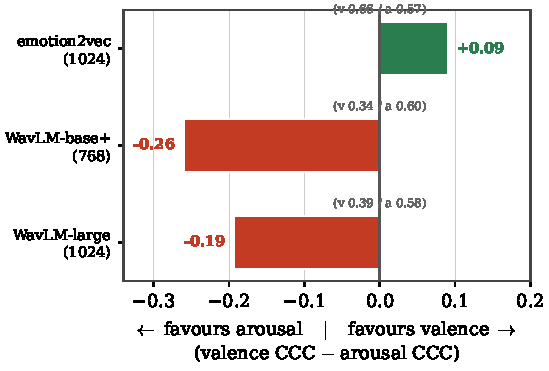
\includegraphics[width=0.9\columnwidth]{figures/fig_encoder.pdf}
\caption{Encoder-specific asymmetry. emotion2vec carries valence best; both WavLM
variants carry arousal better than valence. The split is a property of emotion
pretraining, not size or architecture.}
\label{fig:encoder}
\end{figure}

\subsection{The fix: valence-primary scoring}
Acting on the diagnosis, we compare valence-primary against legacy arousal-based
scoring by the stressed/calm separation $d'$ over all six checkpoints
(Fig.~\ref{fig:dprime}). Valence-primary scoring improves separation on every
checkpoint, with a mean gain of $+0.50$ and a large effect (Cohen's $d = 1.71$;
Wilcoxon signed-rank $p = 0.0312$, near the $n=6$ floor of $0.0156$ and reported
for completeness, not as the main evidence). The gain is consistent in sign and
large in size---the right claim for six paired observations.

\begin{figure}[t]
\centering
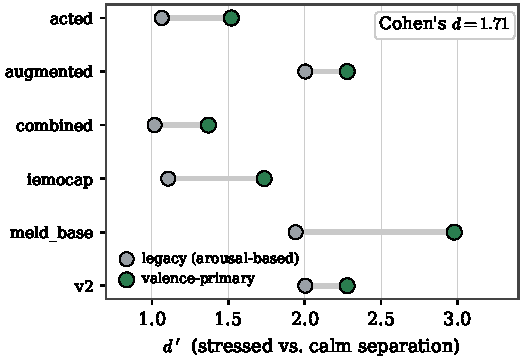
\includegraphics[width=0.92\columnwidth]{figures/fig_dprime.pdf}
\caption{Valence-primary scoring improves stressed/calm separation ($d'$) over
legacy arousal-based scoring for all six checkpoints (Cohen's $d = 1.71$).}
\label{fig:dprime}
\end{figure}

\subsection{Deployment accuracy}
Under leave-one-out thresholding the shipped Fusion-MELD checkpoint reaches
$91.7\%$ on the real-voice set (Table~\ref{tab:deploy}). By language, English
separates without error in this sample ($1.000$, bootstrap $95\%$ CI
$[1.000,1.000]$) and Sinhala reaches $0.909$ ($[0.727,1.000]$). The wide Sinhala
interval follows directly from small sample size and roughly three speakers, so we
do not over-read the point estimate: English is strong and Sinhala is promising but
under-determined, consistent with Sinhala being out of distribution for the frozen
encoder.

\begin{table}[t]
\caption{Deployment accuracy of the shipped model ($n=24$). Overall is
leave-one-out; per-language values are fixed-threshold with bootstrap $95\%$ CIs.}
\label{tab:deploy}
\centering
\setlength{\tabcolsep}{5pt}
\renewcommand{\arraystretch}{1.2}
\begin{tabular}{|l|c|c|c|}
\hline
\textbf{Split} & $\mathbf{n}$ & \textbf{Accuracy} & \textbf{95\% CI} \\
\hline
All (LOO)  & 24 & \textbf{0.917} & $[0.875,1.000]$ \\
\hline
English    & 13 & 1.000 & $[1.000,1.000]$ \\
\hline
Sinhala    & 11 & 0.909 & $[0.727,1.000]$ \\
\hline
\end{tabular}
\end{table}

\section{Discussion}
The five results tell one story. A frozen emotion encoder carries the valence of
real stress reliably but its arousal only weakly, and that asymmetry is what turns
in-domain acted CCC---which rewards arousal agreement on expressive speech---into an
inverted guide for real deployment. Selecting on it favours checkpoints tuned to
the acted high-arousal manifold, and those generalise worst to quiet real stress;
the model trained on naturalistic conversation, weak in-domain, generalises best.
Once stress is read from valence, every checkpoint improves and the ordering stops
hurting.

Why does valence survive the shift and arousal not? Arousal in speech rides mostly
on prosodic energy and pitch dynamics---the very cues an acted delivery exaggerates
and a quiet, internalised speaker suppresses; valence rides on more
distribution-stable tonal and affective qualities that emotion pretraining captures
well. The matched-size probe sharpens the point: the asymmetry belongs to
\emph{emotion} pretraining specifically, not to frozen encoders in general, since
WavLM---pretrained for full-stack speech---shows the opposite bias. The lesson is
not ``always score on valence'' but ``know which axis your encoder transfers, and
score on that.''

The same logic sets bilingual expectations. English is well covered and separates
cleanly; Sinhala is out of distribution, and no scoring rule changes the fact that
the frozen encoder never saw it in pretraining. Rather than overclaim coverage, the
system routes around the limit: voice supplies the valence estimate it can support,
and arousal magnitude comes from the heart-rate-variability module. That is the
right division of labour given the diagnosis, and it is why the paper is a design
as much as a finding.

\section{Limitations and Future Work}
The real-voice set is small ($n = 24$, roughly three Sinhala speakers).
Leave-one-out thresholding removes fit-to-test bias but not small-sample variance,
which is why the per-language intervals are wide and why we lean on the IEMOCAP
replication for inference. Sinhala is out of distribution for the frozen encoder,
and this cannot simply be trained away: adding $26$ Sinhala clips to training
\emph{lowered} held-out accuracy from $90.9\%$ to $81.8\%$---a controlled negative
result showing that more in-language data cannot teach a frozen out-of-distribution
encoder what its pretraining never encoded. In a small three-speaker probe we also
saw a confident single-speaker misread---a quiet accented-English calm clip scored
stressed ($9.13$ at confidence $0.91$); the deployed product mitigates such cases
with a faint-recording confidence guard, a speaker-relative (pre-to-post) verdict,
and deferral to the physiological module, though the exact faint-audio threshold
still awaits calibration on live-test data. Arousal magnitude is unreliable by
design and is offloaded rather than fixed. Finally, Fusion-IEMOCAP is a reference
upper bound, not part of the replication claim. Future work should grow the Sinhala
speaker pool, calibrate the quality gate on live sessions, and test whether a
lightly adapted (rather than fully frozen) encoder can recover arousal for
internalised stress without losing the valence transfer that carries the system
today.

\section{Conclusion}
On real, spontaneous stress, ranking frozen speech-emotion models by their
in-domain accuracy on acted speech is not just uninformative---it is inverted. The
reason is a valence--arousal split: these embeddings carry the valence of real
stress but not its arousal, a pattern we replicate on a large independent corpus
and trace specifically to emotion pretraining. Reading stress from valence rather
than arousal follows directly from the diagnosis and widens stressed/calm
separation on every model we tested, giving a $91.7\%$ leave-one-out detector
deployed bilingually for English and Sinhala, with arousal deferred by design to a
physiological channel. We recommend that future voice-stress systems on frozen
emotion encoders first characterise which affective axis actually transfers to
their deployment distribution, and select and score accordingly, rather than
trusting in-domain acted agreement.

\bibliographystyle{IEEEtran}
\bibliography{references}

\end{document}
